\pagestyle{empty}

% =======================================================
% Capa personalizada (imagem PNG)
% =======================================================
\thispagestyle{empty}
\newgeometry{margin=0cm} % Remove as margens para a imagem preencher a página

\begin{figure}[p]
	\centering
	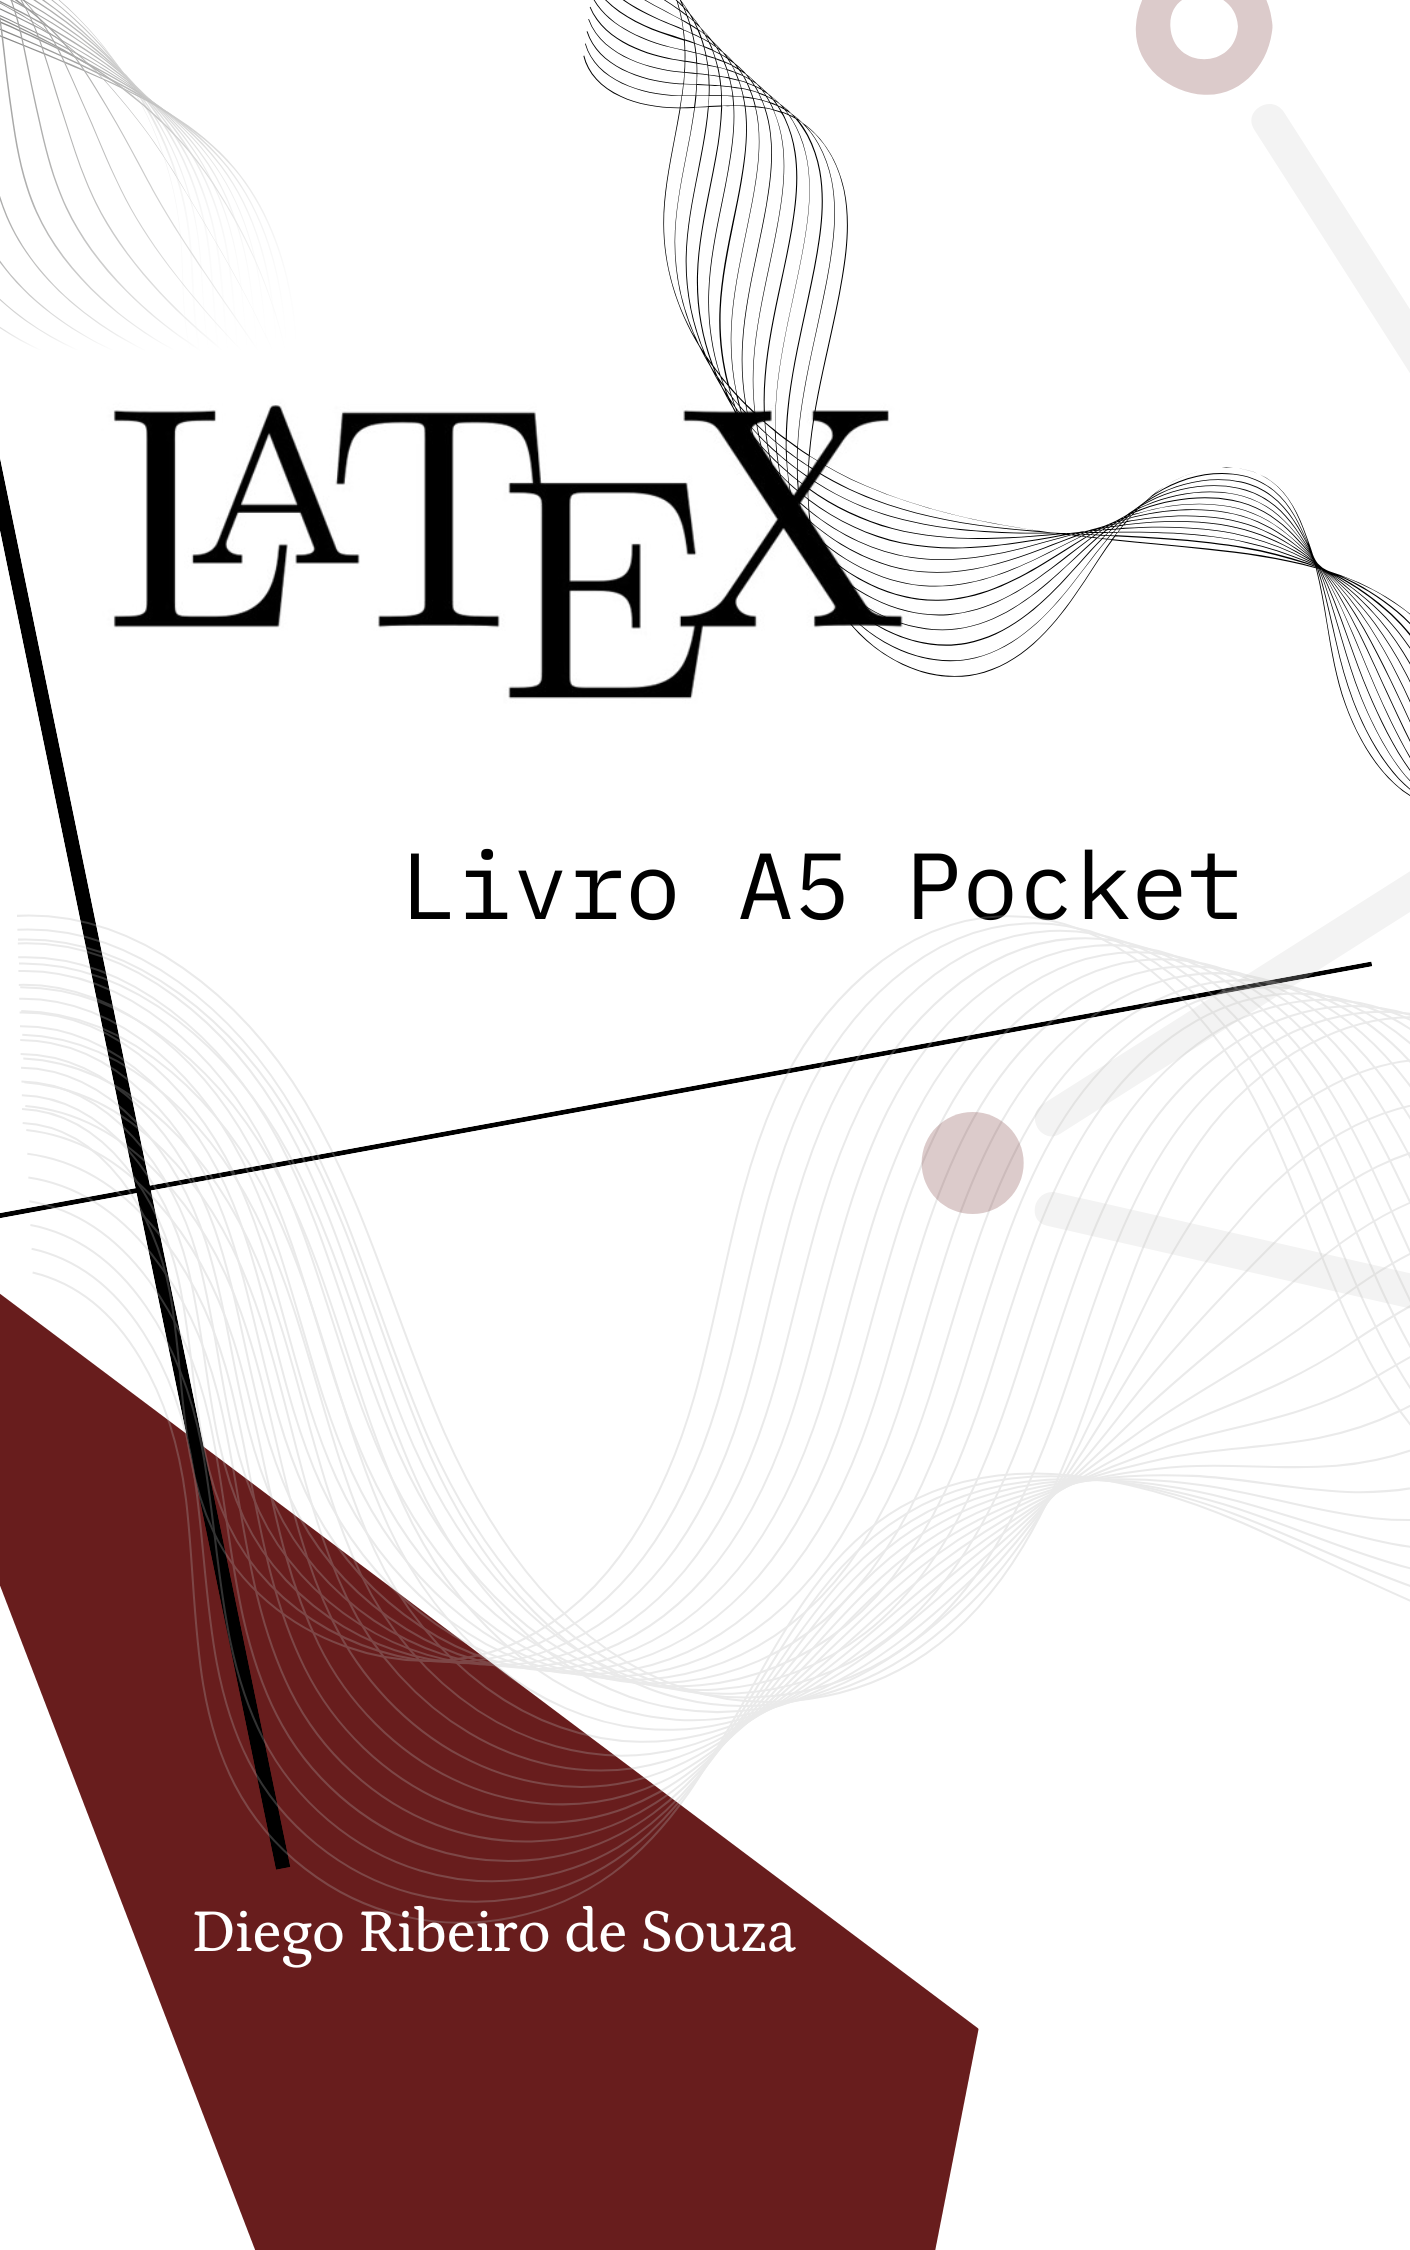
\includegraphics[width=\paperwidth, height=\paperheight, keepaspectratio=false]{/home/diego/Documentos/Livro a5 (pocket) em LaTex (modelo editorial)/frontmatter/Capa.png}
\end{figure}

\restoregeometry % Restaura as margens originais do documento
\cleardoublepage


% =======================================================
% PÁGINA DE TÍTULO (PADRÃO EDITORIAL REFINADO)
% =======================================================
\begin{titlepage}
	\thispagestyle{empty} % Remove o número de página desta folha
	\centering % Centraliza todo o conteúdo horizontalmente
	
	\vspace*{\stretch{2}} % Espaço flexível no topo
	
	% Título do Livro
	{\fontsize{30}{36}\bfseries\booktitle\par} % Título
	\vspace{12pt}
	
	% Subtítulo (se existir)
	\ifx\subtitle\undefined\else
	\if\relax\detokenize\expandafter{\subtitle}\relax\else
	{\large\normalfont\subtitle\par} % Subtítulo
	\fi
	\fi
	
	\vspace*{\stretch{40}} % Espaço flexível entre o título e o autor
	
	% Nome do Autor
	{\authorname\par}
	
	\vspace*{\stretch{6}} % Espaço flexível para empurrar a editora para baixo
	
	% Editora
	{\scshape\publisher\par}
	
	\vfill % Espaço flexível final
\end{titlepage}

% =======================================================
% FICHA CATALOGRÁFICA (COM RODAPÉ NA MESMA PÁGINA)
% =======================================================

\thispagestyle{empty}
\pagestyle{empty}

% Espaço do topo da página para a ficha
\vspace*{1.5cm}

\begin{center}
	% Este minipage grande agrupa toda a ficha e o rodapé
	\begin{minipage}{0.9\textwidth}
		\begin{center}
			{\small\scshape Ficha Catalográfica} \\[10pt]
			{\footnotesize(Conforme Decreto nº 4.591, de 17/12/2002)} \\[10pt]
		\end{center}
		
		\begin{center}
			\fbox{%
				\begin{minipage}{\textwidth}
					\centering
					\footnotesize % Tamanho da fonte para a ficha
					\begin{tabular}{@{}p{\dimexpr\textwidth-2\tabcolsep}@{}}
						\rule{\linewidth}{0.4pt} \\[6pt]
						
						SOUZA, Diego Ribeiro de \\[3pt]
						\hspace{8pt}Filosofia e espiritismo: ensaios sobre os rumos das civilizações / Diego Ribeiro de Souza. -- Ed.~\the\year. -- \publisher, \the\year. \\[3pt]
						\hspace{8pt}\pageref{LastPage}~p. ; 15~cm $\times$ 21~cm \\[6pt]
						
						\hspace{8pt}ISBN: \isbn \\[6pt]
						
						\hspace{8pt}1. Filosofia espírita. 2. Espiritualidade. 3. Metafísica. \\
						\hspace{8pt}4. Espiritismo. I. Título. II. Série. \\[9pt]
						
						CDU: 141.33 \\[6pt]
						\rule{\linewidth}{0.4pt}
					\end{tabular}
					\vspace{9pt}
					\begin{flushright}
						\footnotesize
						\begin{tabular}{r@{}}
							Catalogação na publicação: \\
							Bibliotecária Responsável: \textbf{[Nome Completo]} \\
							CRB-[XX]/[Número] \\
						\end{tabular}
					\end{flushright}
				\end{minipage}
			}
		\end{center}
		
		% Espaçamento entre a ficha e o rodapé
		\vspace*{1cm}
		
		\begin{center}
			\footnotesize % Tamanho da fonte para o rodapé
			\publisher\ -- [Endereço completo] -- Tel.: (XX) XXXX-XXXX \\
			E-mail: contato@editora.com -- www.editora.com.br
		\end{center}
	\end{minipage}
\end{center}

\vfill